\documentclass{beamer}
\usepackage[utf8]{inputenc}
\usepackage{graphicx, epsfig}
\usepackage{amsmath,mathrsfs,amsfonts,amssymb}
\usepackage{floatflt}
\usepackage{epic,ecltree}
\usepackage{mathtext}
\usepackage{fancybox}
\usepackage{fancyhdr}
\usepackage{multirow}
\usepackage{enumerate}
\usepackage{epstopdf}
\usepackage{multicol}
\usepackage{algorithm}
\usepackage[noend]{algorithmic}
\usepackage{tikz}
\usepackage{blindtext}
\usetheme{default}%{Singapore}%{Warsaw}%{Warsaw}%{Darmstadt}
\usecolortheme{default}

\setbeamerfont{title}{size=\Huge}
\setbeamertemplate{footline}[page number]{}

\setbeamertemplate{section in toc}[sections numbered]


\makeatletter
\newcommand\HUGE{\@setfontsize\Huge{35}{40}}
\makeatother    

\setbeamerfont{title}{size=\HUGE}
\beamertemplatenavigationsymbolsempty

% latin bold lower
\newcommand{\ba}{\mathbf{a}} 
\newcommand{\bc}{\mathbf{c}} 
\newcommand{\be}{\mathbf{e}} 
\newcommand{\bh}{\mathbf{h}} 
\newcommand{\bp}{\mathbf{p}} 
\newcommand{\bt}{\mathbf{t}} 
\newcommand{\bs}{\mathbf{s}} 
\newcommand{\bu}{\mathbf{u}} 
\newcommand{\bv}{\mathbf{v}} 
\newcommand{\bw}{\mathbf{w}} 
\newcommand{\bx}{\mathbf{x}} 
\newcommand{\by}{\mathbf{y}} 
\newcommand{\bz}{\mathbf{z}} 

% latin bold upper
\newcommand{\bA}{\mathbf{A}} 
\newcommand{\bB}{\mathbf{B}} 
\newcommand{\bC}{\mathbf{C}} 
\newcommand{\bI}{\mathbf{I}} 
\newcommand{\bJ}{\mathbf{J}} 
\newcommand{\bL}{\mathbf{L}} 
\newcommand{\bM}{\mathbf{M}} 
\newcommand{\bQ}{\mathbf{Q}} 
\newcommand{\bT}{\mathbf{T}} 
\newcommand{\bU}{\mathbf{U}} 
\newcommand{\bV}{\mathbf{V}} 
\newcommand{\bW}{\mathbf{W}} 
\newcommand{\bX}{\mathbf{X}} 
\newcommand{\bY}{\mathbf{Y}} 
\newcommand{\bZ}{\mathbf{Z}} 

% latin cal upper
\newcommand{\cG}{\mathcal{G}} 
\newcommand{\cL}{\mathcal{L}} 
\newcommand{\cN}{\mathcal{N}} 
\newcommand{\cS}{\mathcal{S}} 
\newcommand{\cT}{\mathcal{T}} 
\newcommand{\cW}{\mathcal{W}} 
\newcommand{\cX}{\mathcal{X}} 
\newcommand{\cZ}{\mathcal{Z}} 

% latin bb upper
\newcommand{\bbE}{\mathbb{E}} 
\newcommand{\bbI}{\mathbb{I}} 
\newcommand{\bbP}{\mathbb{P}} 
\newcommand{\bbR}{\mathbb{R}} 

% greek bold lower
\newcommand{\bepsilon}{\boldsymbol{\epsilon}} 
\newcommand{\btheta}{\boldsymbol{\theta}} 
\newcommand{\blambda}{\boldsymbol{\lambda}} 
\newcommand{\bpi}{\boldsymbol{\pi}} 
\newcommand{\bmu}{\boldsymbol{\mu}} 
\newcommand{\bsigma}{\boldsymbol{\sigma}} 
\newcommand{\bphi}{\boldsymbol{\phi}} 

% greek bold upper
\newcommand{\bSigma}{\boldsymbol{\Sigma}} 

\DeclareMathOperator*{\argmin}{arg\,min}
\DeclareMathOperator*{\argmax}{arg\,max}

\newcommand{\createdgmtitle}[1]{\title[\hbox to 56mm{Deep Learning Audio \hfill\insertframenumber\,/\,\inserttotalframenumber}]
	{\vspace{1cm} \\ Deep Learning Audio \\ {\Huge Lecture #1}}
	\author{Pavel Severilov}
	\institute{
	Moscow Institute of Physics and Technology
	} 
	\date{2022}
}

\newcommand\myfootnote[1]{%
  \tikz[remember picture,overlay]
  \draw (current page.south west) +(1in + \oddsidemargin,0.5em)
  node[anchor=south west,inner sep=0pt]{\parbox{\textwidth}{%
      \rlap{\rule{10em}{0.4pt}}\raggedright\scriptsize \textit{#1}}};}

\newcommand\myfootnotewithlink[2]{%
  \tikz[remember picture,overlay]
  \draw (current page.south west) +(1in + \oddsidemargin,0.5em)
  node[anchor=south west,inner sep=0pt]{\parbox{\textwidth}{%
      \rlap{\rule{10em}{0.4pt}}\raggedright\scriptsize\href{#1}{\textit{#2}}}};}
      
\AtBeginSection[]
{
	\begin{frame}{Outline}
		\tableofcontents[currentsection,subsectionstyle=hide]
	\end{frame}
}
\AtBeginSubsection[]{
	\begin{frame}{Outline}
		\tableofcontents[currentsection,currentsubsection]
	\end{frame}
}
\createdgmtitle{4}
\usepackage{tikz}
\usetikzlibrary{arrows,shapes,positioning,shadows,trees}
%--------------------------------------------------------------------------------
\begin{document}
%--------------------------------------------------------------------------------
\begin{frame}[noframenumbering,plain]
%\thispagestyle{empty}
\titlepage
\end{frame}
%=======x
\begin{frame}{Outline}
	\tableofcontents
\end{frame}
%=======
\begin{frame}{ASR: SOTA models}
    \begin{itemize}
        \item RNN-T (2018, Google)
        \item MoChA (2018, Google) (Tricks to make LAS online)
        \item wav2vec (2019, Facebook AI Research) (use WAV not spectrograms)
        \item Jasper (2019, Nvidia) (Encoder – CNN ; Loss: CTC)
        \item QuartzNet (2019, Nvidia) (Encoder – TDS CNN ; Loss – CTC)
        \item ContextNet (2020, Google) (Encoders – CNN and LSTM ; Loss – RNN-T)
        \item Whisper (2022, OpenAi) (Encoder - Transformer; Loss - multitask)
    \end{itemize}
\end{frame}
%=======
\section{RNN-Transducer (RNN-T)}
%=======
\begin{frame}{CTC and Attention models: recap}
\begin{table}[]
\begin{tabular}{|c|c|c|c|}
\hline
\textbf{}                                                    & \textbf{CTC}                                                                                                          & \textbf{\begin{tabular}[c]{@{}c@{}}Listen, Attend \\ and Spell: LAS\end{tabular}}          & \textbf{?} \\ \hline
Summary                                                      & \begin{tabular}[c]{@{}c@{}}Maximize \\ probability of all \\ possible \\ CTC-paths \\ leading to target.\end{tabular} & \begin{tabular}[c]{@{}c@{}}Encoder-decoder \\ architecture \\ with attention.\end{tabular} & ???     \\ \hline
Online  & \textbf{+}   & \textbf{-}  & \textbf{+} \\ \hline
\begin{tabular}[c]{@{}c@{}}Context \\ 
dependent\end{tabular} & \textbf{-} & \textbf{+} & \textbf{+} \\ \hline
\begin{tabular}[c]{@{}c@{}}Multiple outputs \\ 
for each input\end{tabular} & \textbf{-} & \textbf{-} & \textbf{+} \\ \hline
\end{tabular}
\end{table}
\end{frame}

%=======
\begin{frame}{RNN-T: idea}
    \begin{figure}
    	\centering
    	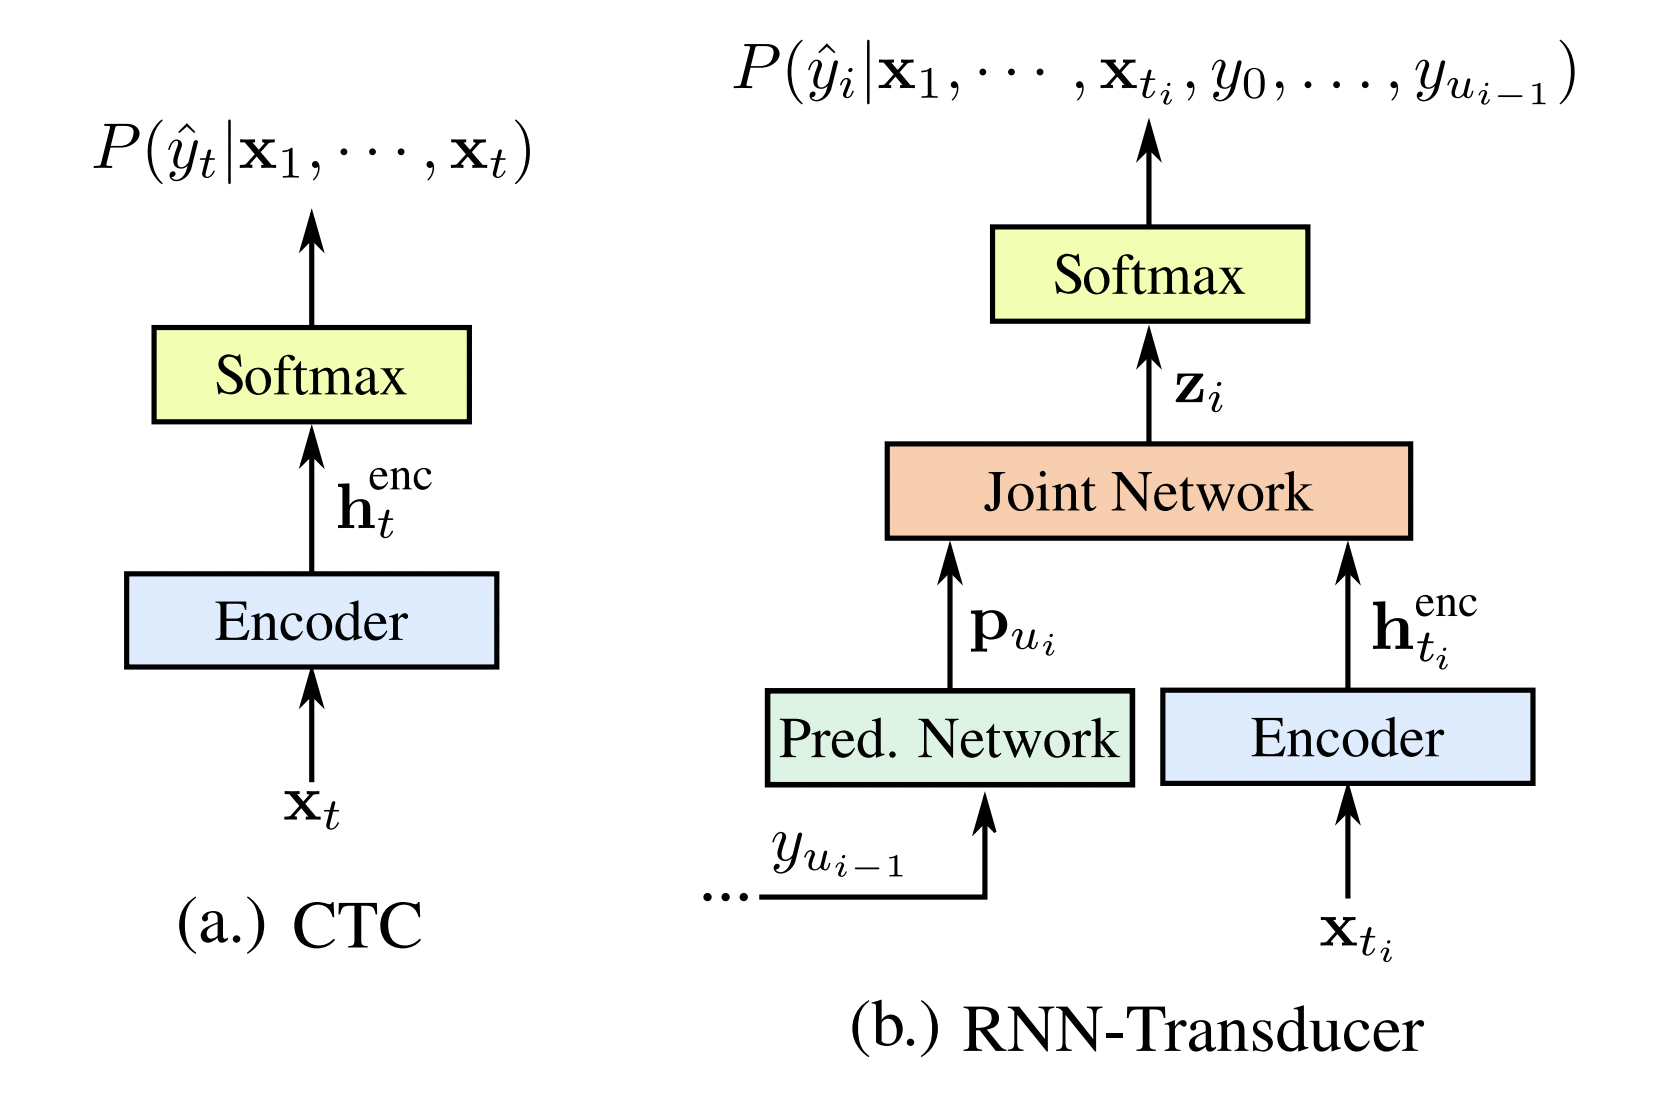
\includegraphics[width=0.75\linewidth]{figs/rnnt.png}
    \end{figure}
    \begin{itemize}
        \item Predictor is autoregressive: takes as input the previous outputs.
        \item Joiner -- feedforward network, combines the encoder vector $h_t$ and predictor vector $p_u$
    \end{itemize}

    \myfootnotewithlink{https://arxiv.org/pdf/1811.06621.pdf}{He et al. Streaming End-to-end Speech Recognition for Mobile Devices / 2019, Google, Inc.}

\end{frame}
%=======
\begin{frame}{RNN-T: model}
    \begin{figure}
    	\centering
    	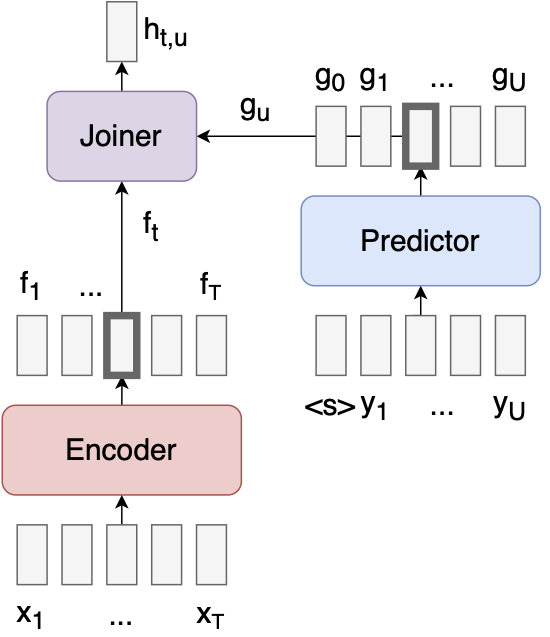
\includegraphics[width=0.55\linewidth]{figs/rnnt_model.png}
    	\caption{RNN-T architecture}
    \end{figure}

    \myfootnotewithlink{https://lorenlugosch.github.io/posts/2020/11/transducer/}{Sequence-to-sequence learning with Transducers blog post}

\end{frame}
%=======
\begin{frame}{RNN-T: model}
    \begin{figure}
    	\centering
    	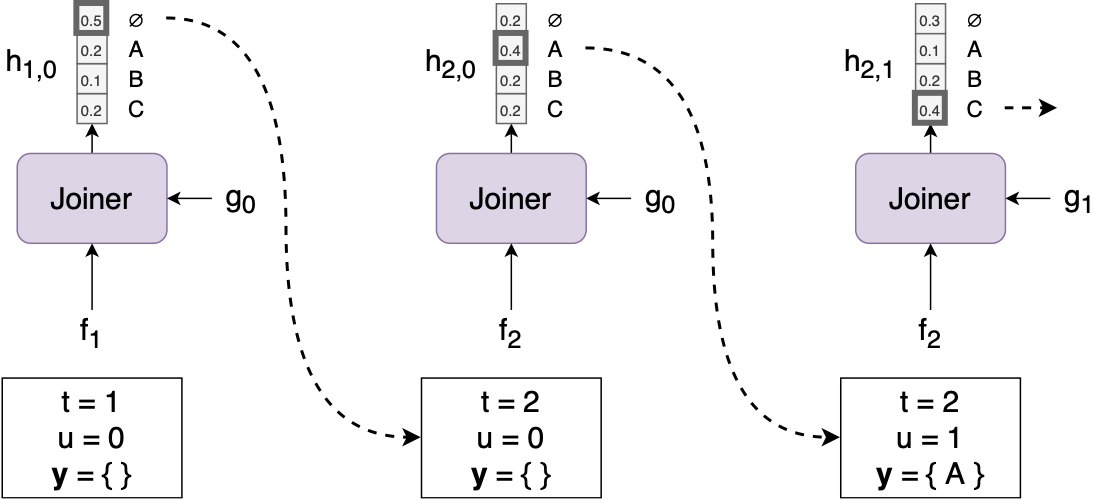
\includegraphics[width=0.99\linewidth]{figs/rnnt_step.png}
    	\caption{Steps example of RNN-T inference: $t$ -- audio-encoder timestamp, $u$ -- Predictor (char network) step}
    \end{figure}
    
    \myfootnotewithlink{https://lorenlugosch.github.io/posts/2020/11/transducer/}{Sequence-to-sequence learning with Transducers blog post}

\end{frame}
%=======
\begin{frame}{RNN-T: training}
    \begin{figure}
    	\centering
    	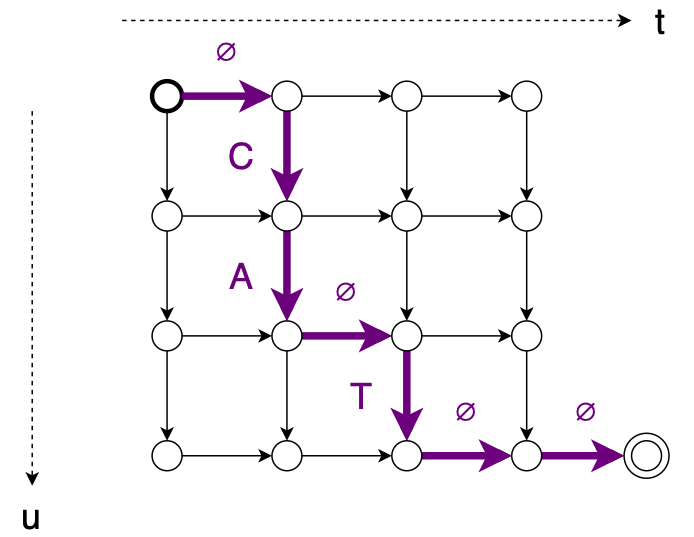
\includegraphics[width=0.8\linewidth]{figs/rnnt_training.png}
    	\caption{Alignment $\{\emptyset, C, A, \emptyset, T, \emptyset, \emptyset\}$ for input sequence of length $T=4$ and an output sequence "CAT" of length $U=3$}
    \end{figure}
    
    \myfootnotewithlink{https://lorenlugosch.github.io/posts/2020/11/transducer/}{Sequence-to-sequence learning with Transducers blog post}
\end{frame}

%=======
\begin{frame}{RNN-T: training}
We need to get $p(\mathbf{y}|\mathbf{x})$ as the sum of the probabilities of all possible alignments between $\mathbf{x}$ and $\mathbf{y}$
    \begin{figure}
    	\centering
    	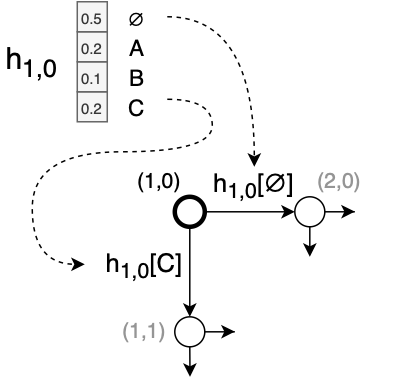
\includegraphics[width=0.5\linewidth]{figs/edge_weights.png}
    	\caption{\begin{aligned}
        &\mathbf{z}=\varnothing, C, A, \varnothing, T, \varnothing, \varnothing \\
        & p(\mathbf{z} \mid \mathbf{x})=h_{1,0}[\varnothing] \cdot h_{2,0}[C] \cdot h_{2,1}[A] \cdot h_{2,2}[\varnothing] \cdot h_{3,2}[T] \cdot h_{3,3}[\varnothing] \cdot h_{4,3}[\varnothing]
        \end{aligned}}
    \end{figure}
    
    \myfootnotewithlink{https://lorenlugosch.github.io/posts/2020/11/transducer/}{Sequence-to-sequence learning with Transducers blog post}
\end{frame}
%=======
\begin{frame}{RNN-T: training}
    To compute the sum efficiently, compute $\alpha_{t, u}$, for $1 \leq t \leq T$ and $0 \leq u \leq U$
    $$
    \begin{array}{r}
    \alpha_{t, u}=\alpha_{t-1, u} \cdot h_{t-1, u}[\varnothing] \\
    +\alpha_{t, u-1} \cdot h_{t, u-1}\left[y_{u-1}\right]
    \end{array}
    $$
    \begin{figure}
    	\centering
    	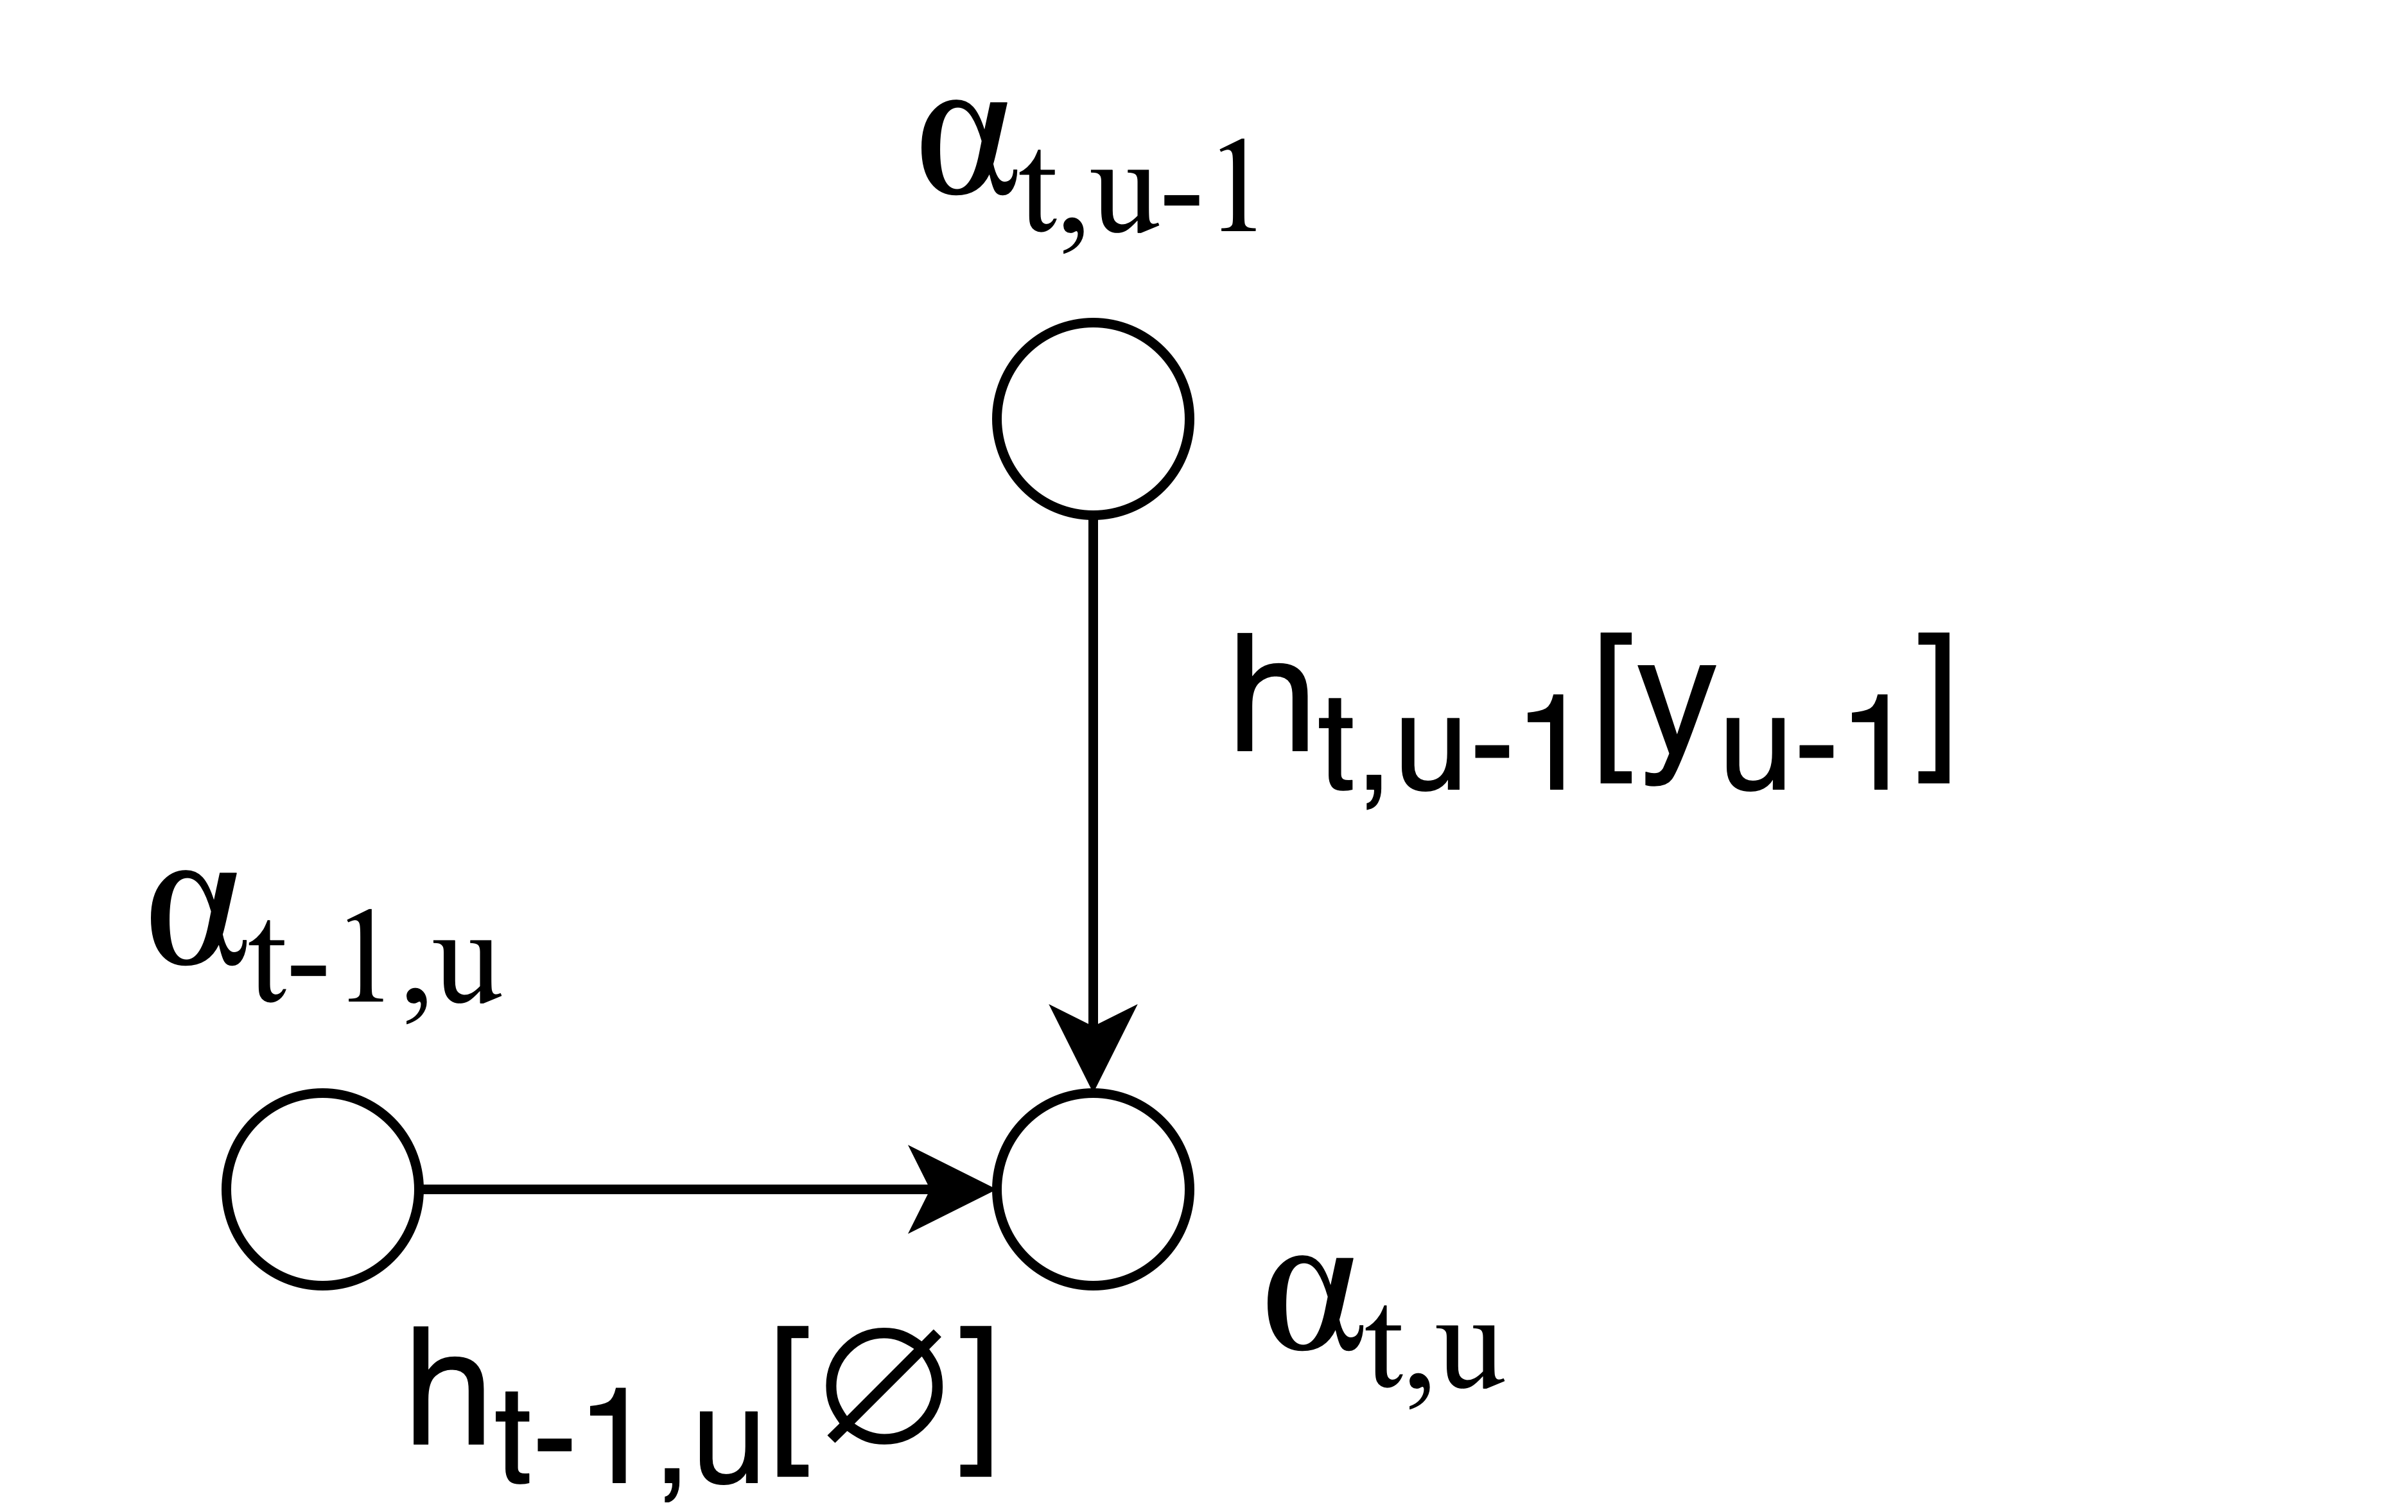
\includegraphics[width=0.5\linewidth]{figs/forward_messages.png}
    	\caption{Computing $\alpha_{t, u}$ to get $p(\mathbf{y} \mid \mathbf{x})=\alpha_{T, U} \cdot h_{T, U}[\varnothing]$} 
    \end{figure}
    
    \myfootnotewithlink{https://lorenlugosch.github.io/posts/2020/11/transducer/}{Sequence-to-sequence learning with Transducers blog post}
\end{frame}

%=======
\section{Language models for ASR}
%=======
\begin{frame}{Language models (LM): why need in ASR?}
\begin{itemize}
    \item Language models recap: a model that estimates the probability of a text.
    \begin{itemize}
        \item N-gramms
        \item Neural networks (BERT, GPT-3, ...)
        \item Example: \\
        $P(\text{let’s go two a movie}) = 0.01$\\
        $P(\text{let’s go to a movie}) = 0.6$
    \end{itemize}
    
    \item ASR problem:
    \begin{itemize}
        \item Spelling of a word heavily depends on its context
        \item Labeled audio data is difficult to obtain
    \end{itemize}

    \item How LM helps: 
        \begin{itemize}
            \item Improves final WER
            \item Improves performance for small audio datasets
            \item Can be used to adapt model to new domain
        \end{itemize}
\end{itemize}
\end{frame}
%=======
\begin{frame}{LM: how to integrate in ASR?}
    \begin{figure}
    	\centering
    	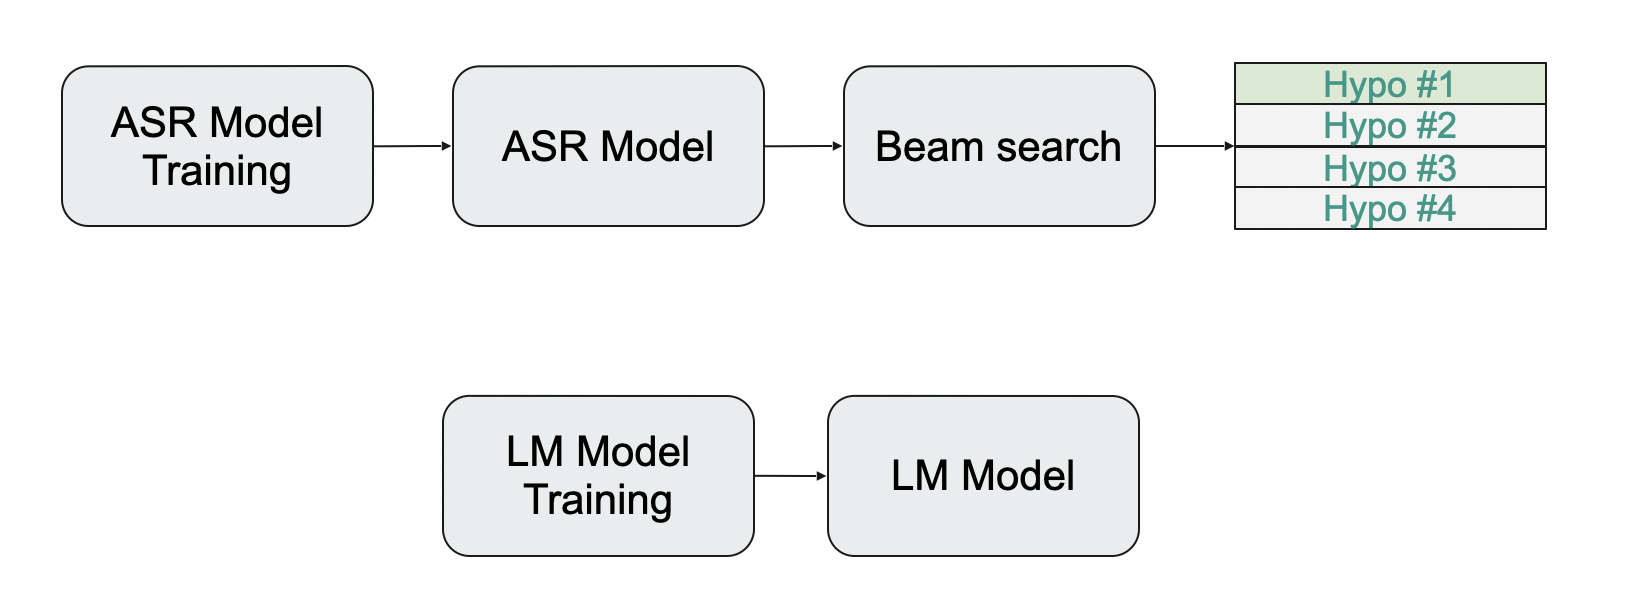
\includegraphics[width=0.99\linewidth]{figs/lm_vs_asr.png}
    	\caption{ASR pipeline VS Language models pipeline}
    \end{figure}
    
    \myfootnotewithlink{https://github.com/markovka17/dla/tree/2020}{HSE DLA course}
\end{frame}
%=======
\begin{frame}{LM: final hypothesis rescoring}
    \begin{figure}
    	\centering
    	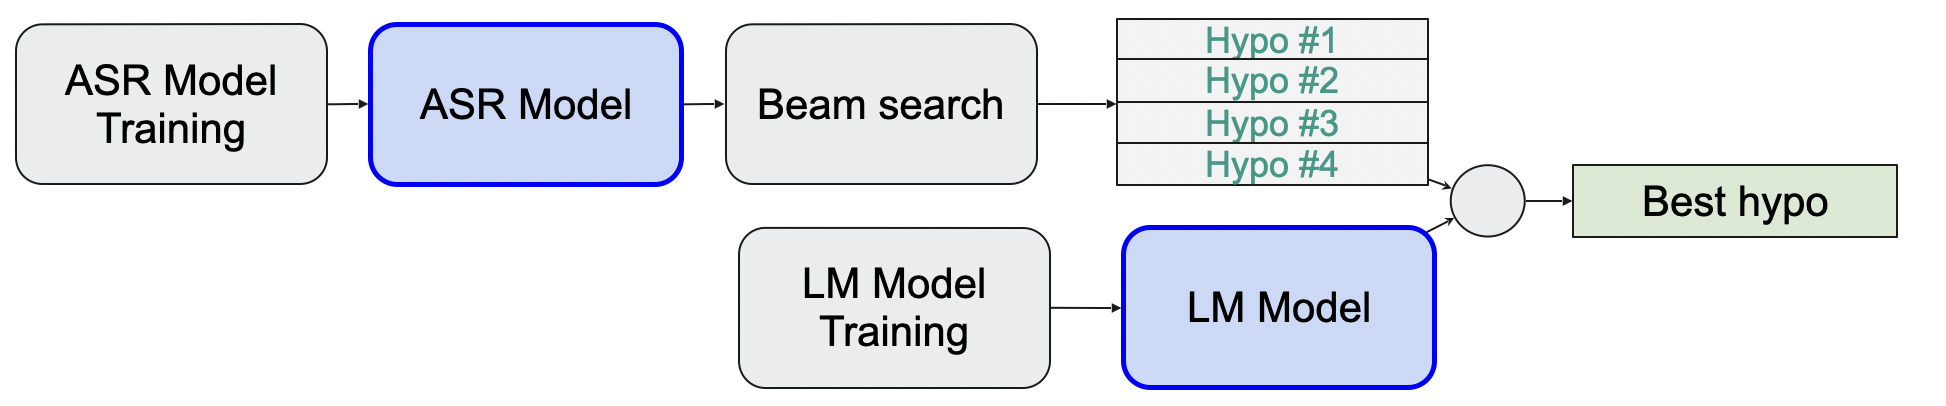
\includegraphics[width=0.99\linewidth]{figs/lm_rescoring.png}
    	\caption{Final hypothesis rescoring: rescore beam-search output with LM probs}
    \end{figure}
    $$\boldsymbol{y}^*=\underset{\boldsymbol{y}}{\arg \max } \log p(\boldsymbol{y} \mid \boldsymbol{x})+\lambda \log p_{L M}(\boldsymbol{y}) +\beta \cdot \operatorname{len}(\boldsymbol{y})$$
    $\operatorname{len}(\boldsymbol{y})$ -- function of word length, anti-penalty for long words
\end{frame}
%=======
\begin{frame}{LM: shallow fusion}
    \begin{figure}
    	\centering
    	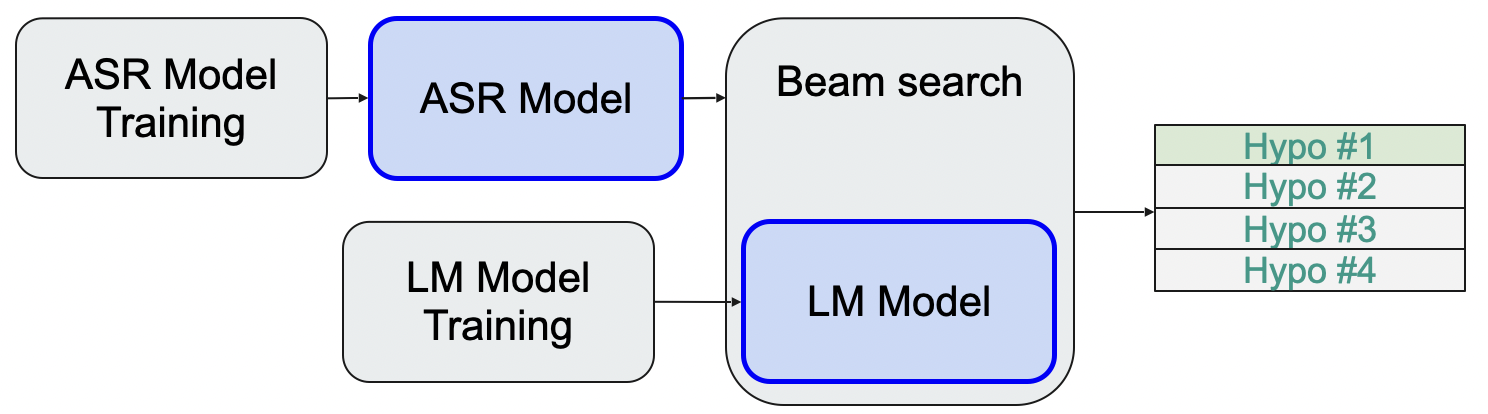
\includegraphics[width=0.99\linewidth]{figs/lm_shallow_fusion.png}
    	\caption{Shallow fusion: use LM rescoring after each beam search step}
    \end{figure}
    Practice: 
    \begin{itemize}
        \item requires much more LM runs
        \item use light LM for shallow fusion
        \item use heavy LM for second-pass rescoring
    \end{itemize}
\end{frame}
%=======
\begin{frame}{LM: Deep fusion}
    \begin{figure}
    	\centering
    	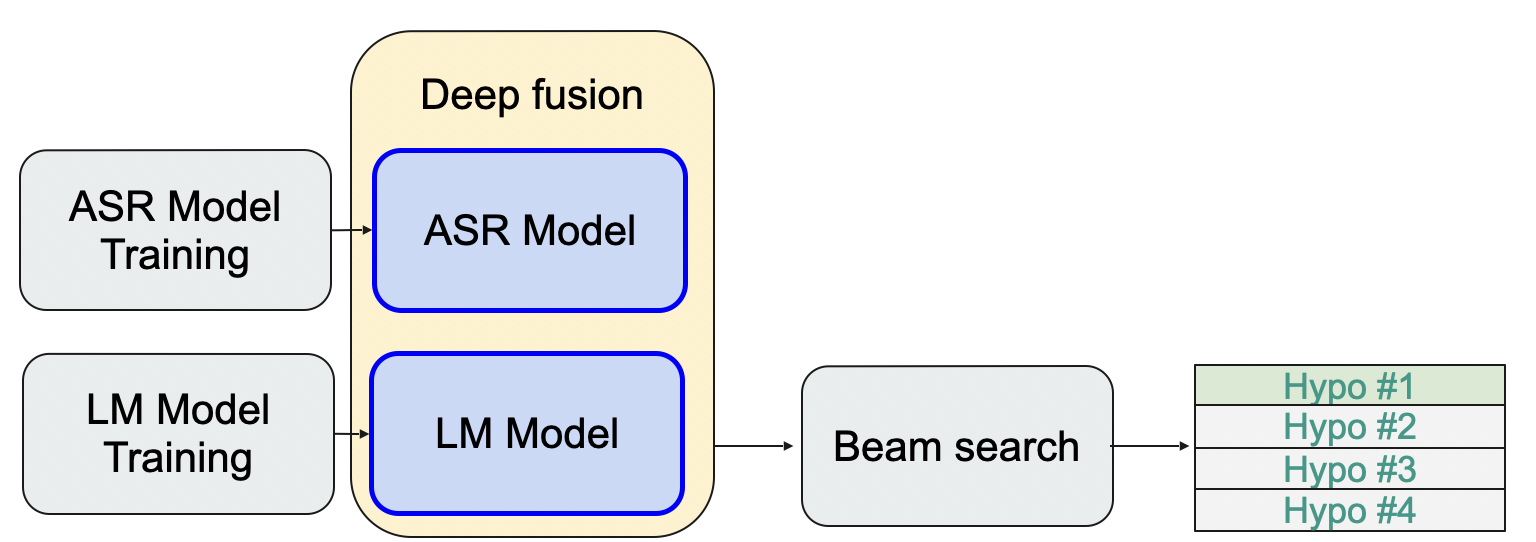
\includegraphics[width=0.99\linewidth]{figs/lm_deep_fusion.png}
    	\caption{Deep fusion: integrates the external LM into the encoder-decoder model (ASR) by fusing together the hidden states of the external LM and the decoder}
    \end{figure}
    
    \myfootnotewithlink{https://arxiv.org/pdf/1807.10857.pdf}{Toshniwal, Shubham et al. “A Comparison of Techniques for Language Model Integration in Encoder-Decoder Speech Recognition.” 2018 IEEE}

\end{frame}
%=======
\begin{frame}{LM: Cold fusion}
    \begin{figure}
    	\centering
    	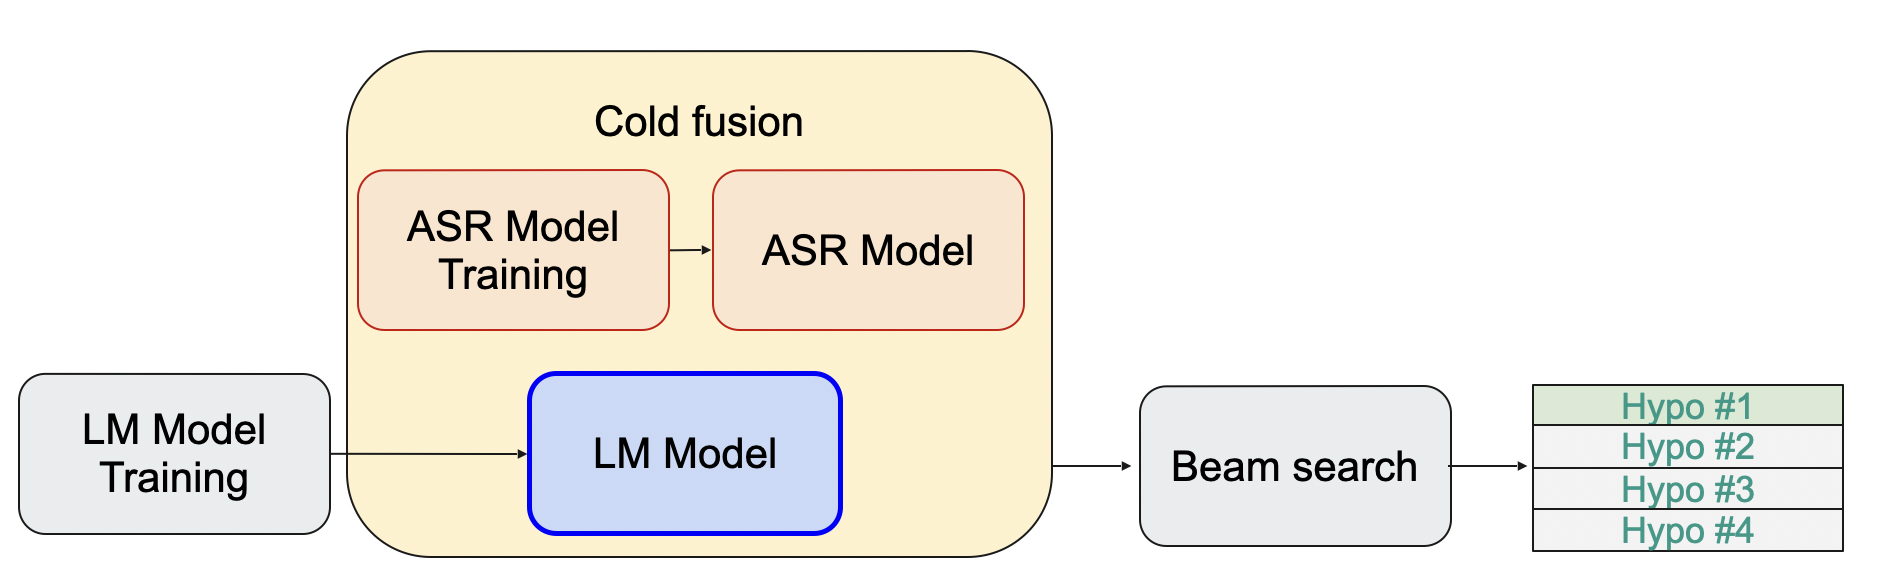
\includegraphics[width=0.99\linewidth]{figs/lm_cold_fusion.png}
    	\caption{Cold fusion: train like in Deep fusion, but jointly with ASR model}
    \end{figure}

    \myfootnotewithlink{https://arxiv.org/pdf/1807.10857.pdf}{Toshniwal, Shubham et al. “A Comparison of Techniques for Language Model Integration in Encoder-Decoder Speech Recognition.” 2018 IEEE}
    \end{frame}
%=======
\begin{frame}{LM in ASR: comparison of approaches}
    \begin{table}[]
        \begin{tabular}{|c|c|c|c|}
        \hline
         \text { Model } & \text { SWB } & \text { CH } & \text { Full } \\
        \hline \text { LAS } & 17.1 & 27.9 & 22.6 \\
        \text { Shallow Fusion } & \textbf{15.6} & \textbf{26.6} & \textbf{21.1} \\
        \text { Deep Fusion } & 16.3 & 27.2 & 21.7 \\
        \text { Cold Fusion } & 16.3 & 27.3 & 21.8 \\
        \hline
        \end{tabular}
        \caption{Word error rates (\%) on Eval2000 for the LAS baseline
        model and fusion approaches. SWB=Switchboard, CH=CallHome,
        Full=Eval2000.}
    \end{table}
    \myfootnotewithlink{https://arxiv.org/pdf/1807.10857.pdf}{Toshniwal, Shubham et al. “A Comparison of Techniques for Language Model Integration in Encoder-Decoder Speech Recognition.” 2018 IEEE}
\end{frame}
%=======
\section{Byte-pair encoding (BPE)}
%=======
\begin{frame}{BPE: motivation \& idea}
\begin{itemize}
    \item Motivation: a lot of characters have different pronunciation in different contexts
    \item Idea: let’s use n-gramms as tokens in addition
    \item Advantages:
    \begin{itemize}
        \item Less decoder steps $\rightarrow$ faster training and inference
        \item Better generalization $\rightarrow$ better WER 
    \end{itemize}
\end{itemize}

\end{frame}
%=======
\begin{frame}{BPE: algorithm}
\begin{enumerate}
    \item Each character -- token
    \item Most popular n-gram: add new token
    \item Replace n-gram with a new token
    \item Restrict maximum length of tokens
    \item New vocabulary = all characters + new tokens
\end{enumerate}
\begin{table}[]
        \begin{tabular}{|c|c|c|}
\hline \text { Iteration } & \text { Sequence } & \text { Vocabulary } \\
\hline 0 & \text { a b a b c a b c } & \{a, b, c\} \\
1 & \text {ab ab c ab c} & \{a, b, c, ab\} \\
2 & \text {ab abc abc} & \{a, b, c, ab, abc\} \\
3 & \text {ababc abc} & \{a, b, c, ab, abc, ababc\} \\
4 & \text {ababcabc} & \{a, b, c, ab, abc, ababc, ababcabc\} \\
\hline
\end{tabular}
\caption{BPE: example for sequence \{ababcabc\}}
    \end{table}


\end{frame}
%=======

\end{document} 
